\documentclass{40k}

\usepackage{pdflscape}

\newcommand{\legacytitle}{CAMPAIGN LEGACY}
\newcommand{\legacystory}{Your must accomplish your quest!}
\newcommand{\legacymissiona}{Any}%
\newcommand{\legacyrolea}{Either}%
\newcommand{\legacymissionb}{Any}%
\newcommand{\legacyroleb}{Either}%
\newcommand{\legacygoal}{CRUSH FACE.}%
\newcommand{\legacybonus}{Hit yourself.}%

\pgfmathsetmacro{\legacycardwidth}{9.25}
\pgfmathsetmacro{\legacycardheight}{12.45}

\newcommand{\legacystripfontsize}{\huge}
\newcommand{\legacycaptionfontsize}{\LARGE}
\newcommand{\legacytextfontsize}{\large}

\newcommand{\legacystriptext}%
  {\legacytitle\hspace{0.5em}\rotatebox[origin=c]{-90}{\includegraphics[width=0.6cm]{icon-skull}}}


%%----------------------------------------------------------------------
%%----------------------------------------------------------------------
\newcommand{\resultstable}{%
\begin{minipage}{\linewidth}%
%\smallskip\centering\legacytextfontsize%
{\bf Campaign Missions:}
\begin{tabular}{C{1.25in}C{1in}c}
  %{\bf Mission} & {\bf Role}&\\% & {\bf Victory}\\
  %\hline
  \legacymissiona & \legacyrolea & \ding{111}\\
  \legacymissionb & \legacyroleb & \ding{111}\\
%  \underline{\hspace{1.25in}} &  \underline{\hspace{1in}} & \ding{111}\\
%  \underline{\hspace{1.25in}} &  \underline{\hspace{1in}} & \ding{111}\\
\end{tabular}%
\end{minipage}%
}


%%----------------------------------------------------------------------
%%----------------------------------------------------------------------
\newcommand{\drawlegacycard}{%
\begin{tikzpicture}%
  \clip (-0.05, -0.05) rectangle (\legacycardwidth+.05, \legacycardheight+.05);

  %%-- Draw the card back and outline
  \draw[rounded corners=\cardroundingradius,fill=white,draw=none] (0,0)
    rectangle (\legacycardwidth,\legacycardheight);
  \node[above left] at (\legacycardwidth+0.1, -0.1)
    {\includegraphics[width=3.5in]{background-skull}};
  \draw[rounded corners=\cardroundingradius] (0,0) rectangle
    (\legacycardwidth,\legacycardheight);

  %%-- Draw the side strip
  \fill[\stripcolor,rounded corners=\striproundingradius]
    (\strippadding,\strippadding) rectangle
    (\strippadding+\stripwidth,\legacycardheight-\strippadding)
    node[rotate=90,above left,white,font=\legacystripfontsize\fontfamily{ptm}\selectfont] {\raisebox{0pt}[15pt][3pt]{\vbox to -18pt{}} \legacystriptext};

  %%-- Draw the player info lines
    \node[text width=(\legacycardwidth-\strippadding-\stripwidth-2*\textpadding)*1cm,
          below right,inner sep=0] at
          (\strippadding+\stripwidth+\textpadding,\legacycardheight-\textpadding)
    {\legacytextfontsize%
      \vbox to 36pt{\it\legacystory}


      \smallskip
      \centerline{\resultstable}

      %\bigskip
      %\centerline{\Large\sc\fontfamily{ptm}\selectfont --- Cataclysm ---}

      \bigskip
      {\bf Cataclysm Goal:} \legacygoal

      \bigskip
      {\bf Campaign Bonus:} \legacybonus
    };

    \node[text width=(\legacycardwidth-\strippadding-\stripwidth-2*\textpadding)*1cm,
          above right,inner sep=0] at
          (\strippadding+\stripwidth+\textpadding,\strippadding)
    {\legacytextfontsize%
      \begin{tabular}{@{}ll}
        \textbf{Name:} &  \underline{\vbox to 18pt{}\hspace{2.125in}}\\
        %\textbf{Squad:} &  \underline{\vbox to 18pt{}\hspace{8.25cm}}\\
        %\textbf{Faction:} & \underline{\vbox to 18pt{}\hspace{8.25cm}}\\
        %\textbf{Alliance:} & \underline{\vbox to 18pt{}\hspace{8.25cm}}\\
      \end{tabular}
    };
\end{tikzpicture}
}

\newcommand{\legacycard}[8]{%
\renewcommand{\legacytitle}{#1}%
\renewcommand{\legacystory}{#2}%
\renewcommand{\legacymissiona}{#3}%
\renewcommand{\legacyrolea}{#4}%
\renewcommand{\legacymissionb}{#5}%
\renewcommand{\legacyroleb}{#6}%
\renewcommand{\legacygoal}{#7}%
\renewcommand{\legacybonus}{#8}%
\drawlegacycard%
}



\begin{document}

%%----------------------------------------------------------------------
%%----------------------------------------------------------------------
\clearpage
\pagetitle{Caldor IV}

\begin{columns}
  

  \emph{Caldor IV} is an unofficial, narrative, team-based, campaign
  tournament for Games Workshop's \emph{Warhammer~40,000}.  Set on the
  long beleaguered world of Caldor IV, the campaign chronicles the
  struggle for \emph{The Scythe Of Unbound Light}, an ancient weapon
  of great might.  It is comprised of three parts:

\begin{squishitemize}
\item \textbf{The Debacle:} Three rounds of standard battles to locate
  critical personnel and ancient weaponry before the planet is
  overrun.

\item \textbf{The Twilight:} Four rounds of~200 point Recon Squad
  skirmishes amid the chaos of the all-consuming, inescapable war.

\item \textbf{The Cataclysm:} A single epic battle encompassing all
  the players, throwing~500 point armies into the maelstrom of the
  planet's final hours as they madly fight to secure \emph{The
    Scythe}.
\end{squishitemize}

The Debacle is playable as a straight tournament with some light team
aspects over it.  The Twilight and Cataclysm are more narrative, but
still have a solid tournament basis.  As such, \emph{Caldor IV}
provides the foundation of a great event for both competition and
narrative oriented players.  The campaign is designed to be played
over two full days or several evenings.

The Twilight and The Cataclysm utilize two additional unofficial
\emph{Warhammer~40,000} supplements:

\begin{squishitemize}
\item \textbf{Recon Squad:} Fast playing, simple rules for skirmish
  level play, in which models move and fight
  individually on heavily terrained boards.

\hfill\url{rocketshipgames.com/games/recon-squad/}\hfill\hbox to 0pt{}

\item \textbf{Cataclysm:} Rules, logistics, and mission scenarios for
  large games comprised of multiple players fighting as teams for
  multiple alliances.

\hfill\url{rocketshipgames.com/games/cataclysm/}\hfill\hbox to 0pt{}
\end{squishitemize}

This document outlines mechanics and missions of the campaign.
Additional tips are on the website:

\hfill\url{rocketshipgames.com/games/caldor-iv/}\hfill\hbox to 0pt{}

\missionheading{Campaign Setup and Overview}

To begin, the players are grouped into two or three alliances,
determined by the organizer(s) based on the factions and number of
players participating:

\begin{squishitemize}
\item \textbf{Forces of Order:} The Imperium and its allies;
\item \textbf{Legions of Discord:} Chaos and heretics;
\item \textbf{Spoilers:} Pirates and xenos of all stripes.
\end{squishitemize}

If only two alliances are warranted by the campaign group, they should
play as Order and Discord.

At the outset of the campaign the Legions of Discord have descended on
Caldor IV en masse in search of \emph{The Scythe Of Unbound Light}, a
lost relic of many legends.  Under siege, the Forces of Order are
about to abandon Caldor IV entirely and scorch everything and everyone
left behind.  First, however, the Mechanicum's Magos Ferdinand,
ranking figure on the world, must be retrieved.  Unaware of the true
stakes, the Spoilers have come simply for bloodshed and whatever they
can plunder.

\end{columns}

\vfill
\begin{story}{1.25in}{Treasure In The Darkness}
  Caldor IV---once a luscious knight world, now a smoldering
  husk. Both The Dark Ages and The Heresy it outlasted, but the
  paranoia and isolation of those times set the kernels of future
  failure.  Over the following eons the houses ossified and turned
  inward, gazing at all about them with mistrust, then fear, and
  eventually war.  Centuries of infighting eventually slagged the
  verdant paradise into a charred wasteland.  In recent centuries the
  Mechanicum has resettled the planet, though their motivations for
  doing so are unclear even as their efforts have increased in recent
  decades.  Intrigued, the planet has since been the target of
  continual raids and exploratory incursions by the more intrepid and
  curious pirates, heretics, and xenos.  Weary, stretched to the
  breaking point, the defense forces have finally all but collapsed
  after decades of unceasing combat.  Sensing the weakness, foes of
  the Imperium have all piled in, lusting for blood or other, more
  secret, goals.  Beseeched by the Mechanicum, loyalists throughout
  the sector have poured in to match, deepening the ever swirling
  maelstrom of the planet-wide conflict.  But time and resources have
  run out.
\end{story}

%%----------------------------------------------------------------------
%%----------------------------------------------------------------------
\clearpage
\pagetitle{The Debacle on Caldor IV}

\begin{columns}

  \emph{The Debacle on Caldor IV} captures the last major thrusts at
  the conclusion of years of fighting over the planet.  All manner of
  allies and foes have come together to fight for whatever spoils
  Caldor IV may yield.

  \missionheading{Goals}

  With new, credible information confirming its existence unearthed
  recently, the Legions of Discord have formed an uneasy alliance
  seeking \emph{The Scythe of Unbound Light}.  This legendary weapon
  has been long since lost to time but is still extant in rumor and
  whispers, believed to be buried amid the planet's vast fields of
  rubble and dunes from its eons of strife.

  The Forces of Order are simply trying to extricate themselves from a
  rapidly worsening quagmire.  Originally the Mechanicum came to the
  planet in search of \emph{The Scythe}, but by this point only fools
  believe it still exists or ever did.  Magos Ferdinand, head of Mars'
  expedition, is such a fool and refused to evacuate until too late.
  Preparations are now underway to obliterate the planet, the
  situation having been deemed irrecoverable by sector governance.
  However, despite his foolish belief in ancient myths, the Magos'
  vast machine knowledge is too valuable to throw away easily. All
  effort necessary should be expended to retrieve him if at all
  possible before Exterminatus.

  Sensing opportunity amid the massive conflict, The Spoilers have
  come simply to smash and grab whatever they can while Order and
  Discord are occupied in a death struggle.  They would be happy to
  lay their claws on either \emph{The Scythe} or Magos Ferdinand.


  \missionheading{Continents}

  Caldor IV has three major continents over which the fighting has
  been concentrated:

  \begin{squishitemize}
  \item \textbf{Apollon:} Heaquarters of the Mechanicum, its primary
    forges, and more mysterious sites...

  \item \textbf{Hermea:} Home to the bulk of the world's civilian
    population in several miserable hive cities.

  \item \textbf{Juno:} Unreclaimed wastelands from the darkest periods
    of the past, not a place to go lightly.
  \end{squishitemize}

  Discord scryers believe \emph{The Scythe} is on Juno but will not
  stake their lives to it.  The precise location is necessary to
  retrieve it anyway.  Magos Ferdinand is assumed to be on Apollon,
  but his location has not been confirmed since the latest heavy
  fighting began.

\columnbreak
\begin{sidestory}{1.7in}{The Debacle on Caldor IV}
  Adept Kain's tentacled machine links withdrew slowly from the
  interface panels surrounding him. He had to cogitate, quietly,
  outside the noostream for a moment. Would this be his failure, or a
  brilliant recovery from failures made by those before him? Magos
  Ferdinand was a fool. This whole expedition had been a
  miscalculation from the start. From the poor research findings Kain
  had reviewed so far, he doubted their quarry had ever been more than
  a myth to begin with. And now the expedition's position had grown
  untenable, with incalculably valuable resources being thrown after a
  madman's quest. Slowly re-interfacing, he assented to the sector
  governor's request for exterminatus. Time to end this throne-cursed
  debacle.
\end{sidestory}

\missionheading{Terrain}

Each continent has a variety of areas represented by the various
tables available: City, industrial, wasteland, and so on.  There are
no specific campaign terrain requirements but players are able to
choose which boards they prefer to defend.  Tables should therefore be
set up in advance and have some distinct characteristics such as more
or less open sight lines and different concentrations of terrain
types.


\missionheading{Missions}

\emph{The Debacle on Caldor IV} is played out over the course of three
missions.  All players contest the same mission in each round.  Almost
any missions can be used, but a tournament ready mission pack is
included in this document following this section.

\missionheading{Setup}

Prepare two sets of three envelopes, one set for Order and the other
for Discord, labelling each for one of the continents on Caldor IV:
Apollon, Hermea, and Juno.  These envelopes capture the alliances'
search for \emph{The Scythe} and the Magos over each continent.

{Print and cut apart the search results cards at the end of this
  section.  Each card indicates an outcome of the alliance's searching
  over a campaign round.}\unskip\parfillskip 0pt \par

\end{columns}

\centerline{
\begin{minipage}[t]{1.0\linewidth}\centering\small\it%
\fbox{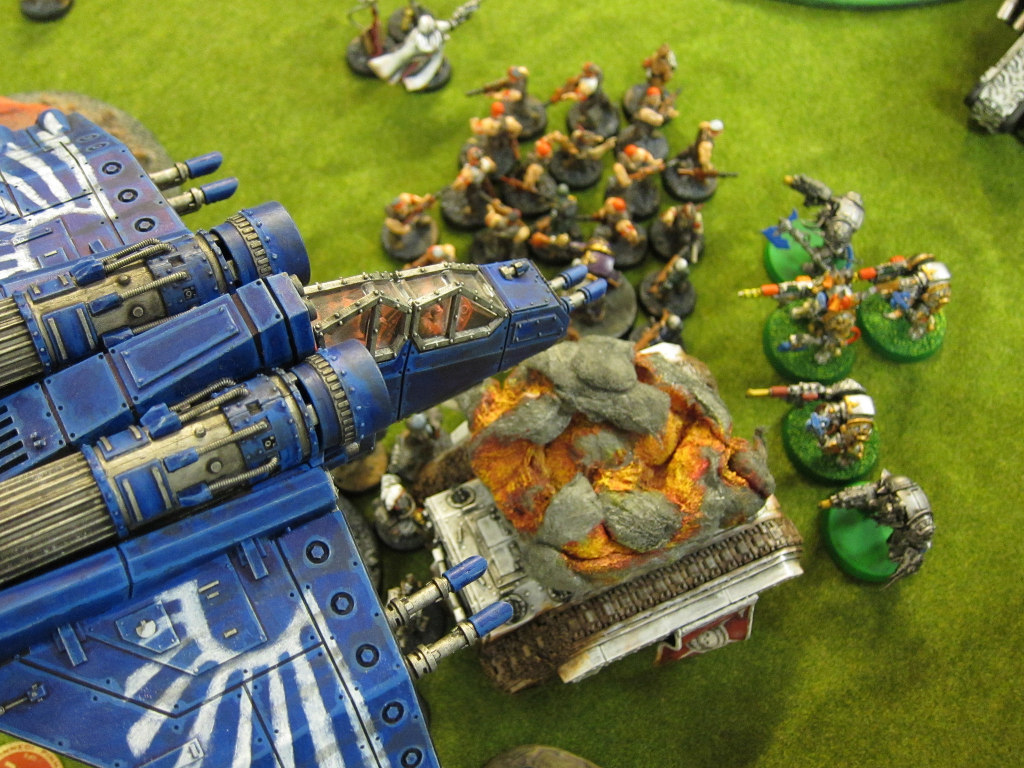
\includegraphics[height=4.5in]{pics/rob-flyer-sm}}\\
Requested air strike imminent on your position.  Take cover.
\end{minipage}
}

\vfill

\begin{columns}

  \noindent%
  Some offer nothing, others reveal the target's continent, and one
  yields their quarry's precise location.

Apply the following procedure for each of the Order and Discord cards.
Organize the numbered cards into four decks, each containing one
``Precise Location'' and two ``Clue'' cards.  Place the decks facedown
and shuffle the set.  Randomly select a deck, discarding the others
without revealing which has been selected.  Keeping the deck facedown,
add the three ``No result'' cards and shuffle the deck.  Without
revealing any contents, for each card randomly select one of its
faction's envelopes and place it inside.

The search envelopes now contain clues to and the precise location of
each alliance's objective, randomly sprinkled across the continents.
Executed carefully, even the organizer(s) won't know where the targets
will be found and may participate as players in the campaign without
compromise.

Finally, print and cut apart a set for each faction of the covert
mission cards at the end of this section.

\missionheading{Campaign Mechanics}

At the end of the three missions, Order and Discord have achieved
their campaign objective if they have discovered the precise location
of their target and control the continent it is on.  The Spoilers
achieve their campaign objective if they know the precise location of
either \emph{The Scythe} or the Magos and control that continent.
Note that the precise location might be discovered on a different
continent from the target's actual location.  This reflects the
worldwide search through ruined libraries, hacked databanks, and
captured individuals eventually yielding the location, which must then
be secured.  If a target's precise location is not found until after
the final round but the alliance ends the campaign in control of that
continent, they still achieve their campaign objective.

Following each round, Order and Discord secretly draw and keep a
search result from their respective envelopes for each continent they
control.  For each continent the Spoilers control they secretly draw
from the envelopes of both Order and Discord, record what they found,
and put the cards back.

Control of a continent is defined as the leader of the accumulated
sums for each alliance of victory points earned in matches held on
that continent.  In event of a tie, each of the tied alliances are
considered to have control.  If the Spoilers are among those tied,
they draw and return their results before the other alliances pull
from their envelopes.

\pagebreak
\missionheading{Round Pairings}

Players are paired with an opponent for each match from another
alliance as best as possible given the number of players.  Teammates
should only battle if no other set of pairings is possible.  In that
rare case, their alliance earns the lesser of the two players' victory
points.  The players though each claim their respective victory points
toward the individual rankings.

First round pairings are randomly assigned across the alliances,
optionally applying a seeding to bias toward matching players of
similar ability.  Starting with the Legions of Discord, then the
Forces of Order, and then the Spoilers, the alliances then alternate
choosing a pairing and assigning it to a continent.  The opposing
alliance responds with a table for that match.

%% (* commander's choice *)
In the second and third rounds, the alliances choose pairings.
Alternating in order by total victory points, each alliance puts
forward a continent and an unmatched player as the attacker.  The
opposing alliance with the most unmatched players in the attacker's
win/loss/draw bracket responds with a defending player and a table for
the match.  If the opposing alliances have an equal number of
unmatched players in the bracket then one alliance is randomly
selected to respond.  The defender must be chosen from the alliance's
unmatched players in the same bracket as the attacker.  If there are
no such players then the defender must be chosen from the closest
possible win/loss/draw bracket.  No two players may ever be matched
more than once.

%% (* random pairings *)
% In the second and third rounds, pairings are assigned randomly across
% the alliances within win/loss brackets as best as possible.  No two
% players may fight more than once, and opponents must be randomly
% selected from within the closest possible win/loss brackets permitting
% that, alternating shifts up and then down the brackets until a match
% is possible.  Proceeding in order by the alliances' total
% campaign-wide victory points and descending down the win/loss
% brackets, the alliances alternate choosing a pairing and assigning it
% to a continent.  The opposing alliance then responds with a table for
% that match.

%% (* tournament pairings *)
% For the second and third rounds, pairings are assigned by win/loss
% brackets as best as possible.  Process each unmatched player in order
% by number of wins, then draws if permitted by the missions, and then
% accumulated victory points.  Assign as their opponent the player from
% another alliance in the same win/draw/loss bracket with the next
% highest victory points that they have not already played.  If there
% are no such players, choose the teammate with the next highest victory
% points from the same bracket that they have not already played.  If
% there are none of those, shift the selection to the next bracket down.
%
% Once pairings are assigned, in order by total victory points the
% alliances alternate choosing a pairing and assigning it to a
% continent.  The opposing alliance then responds with a table for that
% match.

Each continent may only be assigned a limited number of matches per
round: The number of players divided by three and rounded up.  Once
that many matches have been assigned to a continent, pairings may only
be assigned to the other continents.


\missionheading{Covert Missions}

In the second and third rounds, the trailing alliances are given
covert missions to complete and make progress toward their strategic
campaign objectives despite tactical battlefield losses.

Before pairings are assigned to continents for those rounds, the
alliance with the least accumulated victory points secretly draws a
card from its covert mission deck.  Every player in that alliance may
complete the given mission objective in their match to gain the
specified bonus for their alliance.  Following the round that covert
mission is discarded and cannot be selected again, i.e., for the third
round.

In a campaign with three alliances, the middle alliance by accumulated
victory points also draws a covert mission before the second and third
rounds in the same fashion.  However, it may only be attempted by the
half of that alliance's players with the least points, rounding down.


\missionheading{Victory!}

At the conclusion of \emph{The Debacle}, an alliance has won a
campaign victory if it achieved its campaign objective and no other
alliance did as well.  An alliance that controls the majority of the
continents has won a strategic victory.  Finally, the alliance with
the greatest sum total victory points has won a tactical victory.
Each of these outcomes influences the other components of the
\emph{Caldor IV} campaign.  Celebrate the victors, but prepare for the
battles still ahead!

\end{columns}

\pagebreak
\squelchbackground

\begin{landscape}
\vspace*{-15pt}

\noindent%
\searchcard{ORDER SEARCH (1)}{Precise location:\\Apollon,\\Forge Prime.}{The
  Magos is bunkered deep in the bowels of Caldor IV's largest and
  oldest forge with his bodyguards.}\hfill%
\searchcard{ORDER SEARCH (2)}{Precise location:\\Apollon,\\North
  Starport.}{Mechanicum forces are fighting to sustain a desperate
  holdout at the complex in hopes of evacuation.}\hfill%
\searchcard{ORDER SEARCH (3)}{Precise location:\\Hermea,\\Hive
  Pargnosis.}{Witnesses cite the Magos cowering among the
  squalor and innumerable civilians of the lower hab blocks.}\hfill%
\searchcard{ORDER SEARCH (4)}{Precise location:\\Juno,\\The Scar.}{The Magos
  is leading a frantic excavation at the bottom of one of Caldor IV's
  most unnatural features.}

\vfill

\noindent%
\searchcard{ORDER SEARCH (1)}{Clue:\\Apollon.}{A planetary defense company
  saw the Magos board a ground transport near Sub-Forge
  Praxus.}\hfill%
\searchcard{ORDER SEARCH (2)}{Clue:\\Apollon.}{A small group of Skitarii,
  bodyguards of the Magos, were seen fighting on the outskirts of the
  North Starport.}\hfill%
\searchcard{ORDER SEARCH (3)}{Clue:\\Hermea.}{Shuttle pilots logged delivery
  of the Magos' entourage to the continent at the onset of the recent
  fighting.}\hfill%
\searchcard{ORDER SEARCH (4)}{Clue:\\Juno.}{A badly corrupted distress signal\\
  from the Magos' closest protege claims he was headed to The Scar.}

\vfill

\noindent%
\searchcard{ORDER SEARCH (1)}{Clue:\\Apollon.}{Entry records show the Magos
  recently interfaced with the noosphere from a terminal in Sub-Forge
  Maurus.}\hfill%
\searchcard{ORDER SEARCH (2)}{Clue:\\Apollon.}{Requisitions document that the
  Magos ordered an orbital lifter prepared but it was later
  damaged.}\hfill%
\searchcard{ORDER SEARCH (3)}{Clue:\\Hermea.}{Official records indicate the
  Magos had scheduled an oversight meeting with one of the hive
  regents.}\hfill%
\searchcard{ORDER SEARCH (4)}{Clue:\\Juno.}{The expedition's future dimming,
  of late the Magos had been obsessed with several sites in the
  wasteland.}

\vfill

\noindent%
\searchcard{ORDER SEARCH}{No result.}{The Magos' personal logs are recovered
  but are woefully outdated and yield no hint of his location.}\hfill%
\searchcard{ORDER SEARCH}{No result.}{Contact is made with a servant of the
  Magos but the line breaks before they can exchange any
  information.}\hfill%
\searchcard{ORDER SEARCH}{No result.}{None of the senior adepts still alive
  and reachable have seen or heard from the Magos in quite some
  time.}\hfill%
\searchcard{TRASH}{Throw this placeholder card away, it is not used
  in the campaign.}{Thought for the day:\\Sacrifice is best done for
  others.}

\pagebreak

\noindent%
\searchcard{DISCORD SEARCH (2)}{Precise location:\\Juno,\\The Scar.}{Scans
  show \emph{The Scythe} largely intact under mountains of dirt, but
  even if it can be uncovered, will it fly again?}\hfill%
\searchcard{DISCORD SEARCH (1)}{Precise location:\\Juno,\\House
  Etrakus.}{Entombed in rubble, a single alcove in the buried library
  is lit by shafts of light suspending a luminescent blade.}\hfill%
\searchcard{DISCORD SEARCH (3)}{Precise location:\\Hermea,\\Hive
  Pargnosis.}{Deep in the lowest sub-foundation, the mighty war engine
  has quietly powered the entire hive for eons.}\hfill%
\searchcard{DISCORD SEARCH (4)}{Precise location:\\Apollon,\\Forge
  Prime.}{\emph{The Scythe} has lain unrecognized in the Mechanicum's
  vaults for decades, a colossal failure of imagination.}

\vfill

\noindent%
\searchcard{DISCORD SEARCH (2)}{Clue:\\Juno.}{Analysis of radiation patterns
  from metals unburied across the continent point to a spectacular
  crash site.}\hfill%
\searchcard{DISCORD SEARCH (1)}{Clue:\\Juno.}{A burnt data chip plays the
  never before heard saga \emph{The Warsong of Lord Etrakus} and then
  quickly melts.}\hfill%
\searchcard{DISCORD SEARCH (3)}{Clue:\\Hermea.}{A beautiful tapestry
  allegorizes\\\emph{The Scythe} shielding Hermea's houses from
  staggering attacks.}\hfill%
\searchcard{DISCORD SEARCH (4)}{Clue:\\Apollon.}{A faded manifest for
  sub-annex~42A of the original expedition complex lists wonders
  beyond belief.}


\vfill

\noindent%
\searchcard{DISCORD SEARCH (2)}{Clue:\\Juno.}{Only something massive and
  moving incredibly fast could have ripped those gouges into the
  planet.}\hfill%
\searchcard{DISCORD SEARCH (1)}{Clue:\\Juno.}{Stone lythos from the continent
  predating the Imperium depict an illuminated warrior astride the
  world.}\hfill%
\searchcard{DISCORD SEARCH (3)}{Clue:\\Hermea.}{Early texts chart the lineage
  of the population centers back to the survivors of the founding
  houses.}\hfill%
\searchcard{DISCORD SEARCH (4)}{Clue:\\Apollon.}{An empty docking interface
  for \emph{The Scythe} is found, with Mechanicum extraction equipment
  nearby.}\hfill%

\vfill

\noindent%
\searchcard{DISCORD SEARCH}{No result.}{The long sought-for vault's\\contents
  begin crumbling immediately upon exposure to atmosphere.}\hfill%
\searchcard{DISCORD SEARCH}{No result.}{ Only false beliefs and nonsense spew
  from the hoary integrated librarian before you end his
  delusions.}\hfill%
\searchcard{DISCORD SEARCH}{No result.}{Your servants are imbeciles, useful\\
  as little more than scrap meat.}\hfill%
\searchcard{TRASH}{Throw this placeholder card away, it is not used in
  the campaign.}{Thought for the day:\\Sacrifice is best done by
  others.}

\end{landscape}

\pagebreak%

\noindent%
\covertcard%
{Interrogation}%
{Command has ordered you to capture and interrogate prisoners.  It's
  against your usual ``No mercy'' philosophy, but they're in charge.}%
{After all deployment concludes, secretly select and record an enemy
  character.  You succeed if that character is removed as a casualty
  and you pass a~D6 test against its role:

\bigskip
\begin{minipage}{1.0\linewidth}\centering
\textbf{HQ} 2+ ~~ \textbf{Elite} 3+ ~~ \textbf{Troop} 5+\\
\textbf{Fast} 4+ ~~ \textbf{Heavy} 4+  
\end{minipage}}%
{Your alliance pulls a search result for each continent on which a
  player achieved this mission as though it shared control.}
%{For each player in your alliance that passes this test, the alliance
%  of their opponent shares its search results so far with yours after
%  results are drawn this round.}%
\hfill%
\covertcard%
{Sweep \& Scan}%
{Your troops are on the roll, rapidly covering ground in the hunt for
  intel.  You might miss something moving so fast, but time's up.}%
{At the end of each of your turns beginning with Turn~2, secretly make
  a note for each primary objective marker outside your deployment
  zone which you control and have not previously controlled.  If by
  the end of the game you have controlled at least two at some point,
  you succeed.}%
{Your alliance pulls a search result for each continent on which a
  player achieved this mission as though it shared control.}

\vfill

\noindent%
\covertcard%
{Data Port}%
{You've detected an active, unsecured data port among the wreckage
  strewn about.  If you can hold it long enough, you might be able to
  extract something useful.}%
{After all deployment concludes, secretly select and record a primary
  objective marker outside your deployment zone.  You succeed if you
  control it at the end of your turn for any two turns in a row,
  excluding Turn~1.}%
{In addition to the points you earn as usual, your alliance gains half
  the maximum victory points possible for this match toward its
  overall and this continent.} \hfill%
\covertcard%
{Signals}%
{You're tracking an enemy HQ signal.  If you can triangulate it,
  you'll know where they're based.}%
{After all deployment concludes, secretly select and record a table
  quarter not on your table edge.  At game end if you have a scoring
  unit in that quarter and your opponent does not, you succeed.  Units
  with Objective Secured trump those without.}%
{In addition to the points you earn as usual, your alliance gains half
  the maximum victory points possible for this match toward its
  overall and this continent.}

\pagebreak
\restorebackground%

%\vfill
%\noindent%
%\begin{minipage}[t]{1.0\linewidth}\centering\small\it%
%\fbox{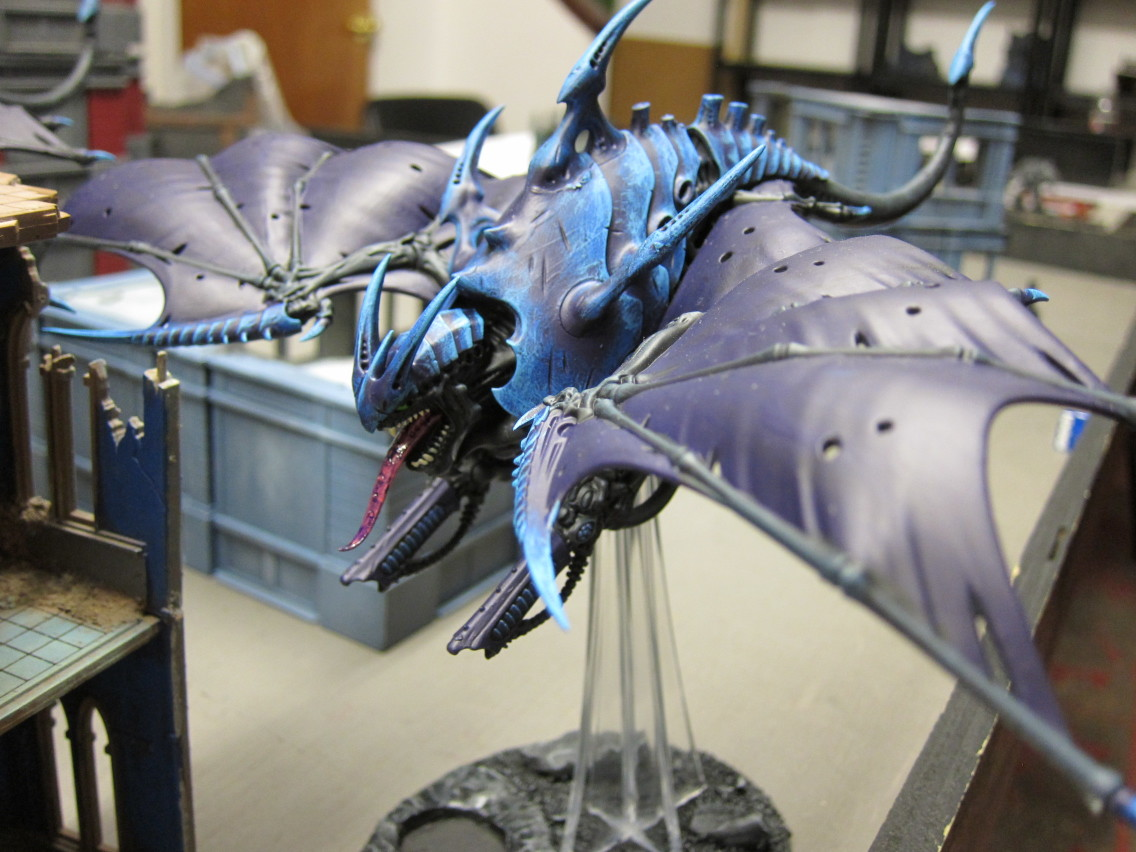
\includegraphics[width=(1.0\linewidth)]{pics/IMG_9230-sm}}\\
%Scour the skies!
%\end{minipage}

%%----------------------------------------------------------------------
%%----------------------------------------------------------------------
\clearpage
\pagetitle{The Debacle: Mission Pack}

\begin{columns}

\missionheading{Army Construction}

Armies must be selected to at most~1500 points.  All up to date
sources\footnote{Partial list maintained by Redcap's Corner and PAGE:
  \url{http://bit.ly/1uWkFHz}} are permitted.  No requirements or
constraints are placed on detachments or force organizations.  Forge
World units and armies eligible for standard \emph{Warhammer 40,000}
are permitted.

Models need not be painted, but objective painting scores will be
applied to reward finished armies.

Models must be WYSIWYG, but identifiable and thoughtful conversions
are welcome.  Contact the tournament organizer(s) beforehand about any
uncertain models.  ``Counts-as'' proxies and undistinguishable or
confusing stand-ins are not permitted.

\missionheading{Supporting Materials}

You must have an official, legal, complete physical or digital copy on
hand for all army, unit, and other sources you are using.  You should
bring printed copies of relevant pages of any electronic sources.
Don't forget errata and FAQs for your sources.\footnote{Available from
  The Black Library:
  \url{http://www.blacklibrary.com/faqs-and-errata.html}}

You must bring any dice, templates, and markers you need to facilitate
playing your army, as well as five typed copies of your army roster
with points listed.


\missionheading{Startup Sequence}
Each mission will use the following setup process:

\begin{itemize}\shortlist
\item Clarify terrain and exchange lists

\item Determine warlord traits, then psychic powers, and then other
  pre-game effects and choices

\item D6 roll off to select deployment zones

\item Place primary objective markers

\item D6 roll off to choose first or second deployment

\item Deploy main armies in that order

\item Deploy any Infiltrators (pg. 167)

\item Secretly choose and record secondary objectives from the options
  listed for the mission

\item Make any Scout redeployments (pg. 171)

\item Reveal secondary objectives

\item First to deploy chooses to play first or second

\item Seize the Initiative roll, if desired

%\item \emph{Fight!}
\end{itemize}

\columnbreak

\missionheading{Mission Rules}%

The following special rules will be applied to each mission, in
addition to any given by the mission definition or otherwise
specified, e.g., for a particular table.

\missionsubheading{Easy Recon.}  Players add~+1 to their roll to
choose first or second deployment for each superheavy vehicle or
gargantuan creature in the opposing army.

\missionsubheading{Reserves.} As defined on page~135 of the main
\emph{Warhammer 40,000} rulebook.

\missionsubheading{Seize the Initiative.} As defined on page~132 of
the main \emph{Warhammer 40,000} rulebook.

\missionsubheading{Variable Game Length.} As defined on page~133 of
the main \emph{Warhammer 40,000} rulebook.

\missionsubheading{All In.}  Units/models in reserve at game end count
as completely destroyed/removed as a casualty.

\missionheading{Scoring}%

Match results are determined by scoring primary, secondary, and
tertiary objectives as given for each mission.  Any unit or faction
specific rules granting victory points \emph{to a player's opponent}
also apply.

The winner of a match is the player with the most victory points.
Ties are broken in favor of the player with the most army points on
the table at game end, including embarked units and claimed
fortifications.

Tournament standings are determined first by win/loss records and then
the sum total victory points achieved across all three missions.  No
more than~20 victory points may be earned per mission toward these
standings, though any additional victory points won do count toward
determining the match winner.

\vfill
\begin{story}{24pt}{The Demands of Thirsty Gods}
  Carragon stood for a moment after the voice in his head faded away.
  Even by the standards of his pirate band this last request was
  excessive, unnecessary.  But the rewards...
\end{story}

\end{columns}

%%----------------------------------------------------------------------
%%----------------------------------------------------------------------
\missiontitle{Mission 1: Contact}

\centerline{\emph{Armies collide as the vanguards of opposing sides
    make contact in the burgeoning planetary war.}}

\missionheading{Table Setup}

Deployment zones are \textbf{Vanguard Strike}, as defined on page~131
of the main \emph{Warhammer 40,000} rulebook.  Vanguard Strike may be
approximated by deploying within a 33.5'' x 50'' table corner
triangle.  The player that wins the zone roll off may pick any of the
four corners, and the other player takes that diagonally opposite.

\bigskip%
After determining deployment zones, place one primary objective marker
at the center of the table and one at each of the two table quadrant
centers outside the deployment zones, i.e., 18'' from the short table
edge and 12'' from the long table edge in the corners opposite the
deployment zones.  There are thus three primary objective markers
along the diagonal dividing the no man's land between the two
deployment zones.

\missionheading{Mission Specific Rules}

The following mission specific rules apply, in addition to those
applied to all missions in this pack.

\missionsubheading{Nightfighting.}  All units have Stealth on Turn 1.

% As defined on page~135 of the main
% \emph{Warhammer 40,000} rulebook.


\missionheading{Scoring}

This mission is scored by objectives achieved, as follows.

\missionsubheading{Primary Objectives.} At the conclusion of the game,
players score~3 victory points for each primary objective marker they
control, as defined by the standard rules (page~134 of the main
rulebook).


\missionsubheading{Secondary Objectives.}

After deployment, both players simultaneously choose and then reveal a
single secondary objective for themselves from the list below.  Any
necessary selections are chosen and then revealed with the objective
unless noted otherwise.  \underline{No more than~6 victory points may
  be earned via any secondary.}

\begin{itemize}
\item \textbf{Seek and Destroy.}  Choose and declare a Battlefield
  Role other than Troop.  Score~2 victory points for each enemy unit
  of this role completely destroyed or falling back at the end of the
  game.

\item \textbf{Victory Through Attrition.}  Score~1 victory point for
  each unsaved hull point or wound taken from any opposing superheavy
  vehicle or gargantuan creature by any means, including explosions
  and other indirect effects.  These points are earned at the end of
  any phase in which such damage occurs, and thus include any repaired
  or regenerated later.

\item \textbf{Seize Ground.}  Choose two terrain pieces not in your
  deployment zone.  Do not declare these now, but do secretly record
  your selection unambiguously!  Reveal these at game end and score~3
  victory points for each piece that you control, treating them as
  objective markers.  Note that this means a single unit cannot claim
  both a primary objective marker and a terrain piece simultaneously.

\item \textbf{Reconnaissance.}  At the end of the game, score~2
  victory points for each friendly scoring unit with the Scout or
  Infiltrate USR completely within 12'' of your opponent's table edge.

\end{itemize}


\missionsubheading{Tertiary Objectives.}  Both players apply all of
the following tertiary objectives:

\begin{itemize}
\item \textbf{Slay the Warlord.}  If the opposing army has a Lord of
  War character or a Warlord of any type and either has been removed
  as a casualty or is falling back at the end of the game, score~2
  victory points.

\item \textbf{Linebreaker.}  Score~2 victory points if a model from
  any friendly scoring unit is completely within 12'' of your
  opponent's table edge.

\item \textbf{First Blood.}  As defined on page~133 of the main
  \emph{Warhammer 40,000} rulebook.
\end{itemize}


%%----------------------------------------------------------------------
%%----------------------------------------------------------------------
\missiontitle{Mission 2: Ground At Any Cost}

\centerline{\emph{Warriors lock into combat as they desperately fight
    to carve out space for their army on the battlefield.}}

\missionheading{Table Setup}

Deployment zones are \textbf{Dawn of War}, as on page~131 of the
\emph{Warhammer 40,000} rulebook (12'' long edges).

\bigskip%
After determining deployment zones, six primary objective markers are
put down.  Each player receives three markers which they alternate
placing, beginning with the winner of a D6 roll off, in the following
order:

\begin{itemize}
\item Your first marker is worth~3 victory points and must be placed
  in either deployment zone.

\item Your second marker is worth~2 victory points and must be placed
  in the opposite zone from your first.

\item Your third marker must be placed on the table centerline, i.e.,
  anywhere 24'' from both long edges.
\end{itemize}

All other placement rules apply as given on page~134 of the main
\emph{Warhammer 40,000} rulebook.  After placement, randomly select
one of the two centerline markers to be worth~4 victory points.  The
other centerline marker is worth~1 victory point.  Make sure to
unambiguously record the value of all markers.


\missionheading{Mission Specific Rules}

There are no mission specific rules for this mission.


\missionheading{Scoring}

This mission is scored by objectives achieved, as follows.

\missionsubheading{Primary Objectives.} At the conclusion of the game,
for each primary objective marker a player controls they score the
number of victory points it is worth as determined during table setup.

\missionsubheading{Secondary Objectives.}

There are no secondary objectives for this mission.

\missionsubheading{Tertiary Objectives.}  Both players apply all of
the following tertiary objectives:

\begin{itemize}
\item \textbf{Slay the Warlord.}  If the opposing army has a Lord of
  War character or a Warlord of any type and either has been removed
  as a casualty or is falling back at the end of the game, score~2
  victory points.

\item \textbf{Linebreaker.}  Score~2 victory points if a model from
  any friendly scoring unit is completely within 12'' of your
  opponent's table edge.

\item \textbf{First Blood.}  As defined on page~133 of the main
  \emph{Warhammer 40,000} rulebook.
\end{itemize}


%%----------------------------------------------------------------------
%%----------------------------------------------------------------------
\missiontitle{Mission 3: The Final Grind}

\centerline{\emph{Tired, near breaking, armies make desperate gambles
    in the waning throes of conquest or defeat.}}

\missionheading{Table Setup}

Deployment zones are \textbf{Hammer and Anvil}, as defined on page~131
of the main rulebook (24'' short edges).

\bigskip%
In each of the four table corners place a primary objective marker
12'' from both of the table edges of that corner.  Place a fifth
primary objective marker at the center of the table.

\missionheading{Mission Specific Rules}

The following mission specific rules apply, in addition to those
applied to all missions in this pack.

\missionsubheading{The Longest Day.}  After Turn~4 roll a D6; on a~4+
all units have Stealth for the remainder of the game.  Do this again
after Turn~5 if it did not take effect.  This rule automatically takes
effect after Turn~6.


\missionheading{Scoring}

This mission is scored by objectives achieved, as follows.

\missionsubheading{Primary Objectives.} At the conclusion of the game,
players score~2 victory points for each primary objective marker they
control in a table corner, and~1 victory point for controlling the
marker at table center.



\missionsubheading{Secondary Objectives.}

After deployment, both players simultaneously choose and then reveal a
single secondary objective for themselves from the list below.  Any
necessary selections are chosen and then revealed with the objective
unless noted otherwise.  \underline{No more than~6 victory points may
  be earned via any secondary.}

\begin{itemize}
\item \textbf{Seek and Destroy.}  Choose and declare a Battlefield
  Role other than Troop.  Score~2 victory points for each enemy unit
  of this role completely destroyed or falling back at the end of the
  game.

\item \textbf{Victory Through Attrition.}  Score~1 victory point for
  each unsaved hull point or wound taken from any opposing superheavy
  vehicle or gargantuan creature by any means, including explosions
  and other indirect effects.  These points are earned at the end of
  any phase in which such damage occurs, and thus include any repaired
  or regenerated later.

\item \textbf{Meatgrinder.}  Score~1 victory point for each opposing
  Troop unit completely destroyed or falling back at the end of the
  game.

\item \textbf{Assassination.}  Score~1 victory point for each opposing
  character model removed as a casualty or falling back at the end of
  the game.  Note that this is not limited to just independent
  characters.

\end{itemize}


\missionsubheading{Tertiary Objectives.}  Both players apply all of
the following tertiary objectives:

\begin{itemize}
\item \textbf{Slay the Warlord.}  If the opposing army has a Lord of
  War character or a Warlord of any type and either has been removed
  as a casualty or is falling back at the end of the game, score~2
  victory points.

\item \textbf{Linebreaker.}  Score~2 victory points if a model from
  any friendly scoring unit is completely within 12'' of your
  opponent's table edge.

\item \textbf{First Blood.}  As defined on page~133 of the main
  \emph{Warhammer 40,000} rulebook.
\end{itemize}


\pagebreak
\pagetitle{The Twilight of Caldor IV}

\begin{columns}

  \emph{The Twilight of Caldor IV} is played as four rounds of Recon
  Squad skirmishes between 200 point armies.  Full rules for Recon
  Squad are available here:

\centerline{\url{rocketshipgames.com/games/recon-squad/}}

\end{columns}

%%----------------------------------------------------------------------
%%----------------------------------------------------------------------
\vfill
\noindent
\begin{minipage}[t]{1.0\linewidth}\centering%
\rowcolors{2}{gray!12}{white}\setlength{\tabcolsep}{3pt}%
\begin{tabular}{|l|c|c|c|c|c|c|c|c|}
\hline
\rowcolor{gray!25} {\bf Mission}       & {\bf Explorators} & {\bf Harriers} & \begin{tabular}[b]{@{}c@{}}\bf Quarter-\\\bf masters\end{tabular} & {\bf Rampagers} & {\bf Sentinels} & {\bf Penetrators} & {\bf Survivors} & {\bf Warriors}\\
%\bf Mission}       & {\bf Explorators} & {\bf Harriers} & {\bf Quartermasters} & {\bf Rampagers} & {\bf Sentinels} & {\bf Penetrators} & {\bf Survivors} & {\bf Warriors}\\
\hline
\hline
{\bf Artifact}      & Either            &                & Either               &                 &                 &                &                 &               \\
{\bf Assassination} &                   & Attacker       &                      &                 &                 &                & Defender        &               \\
{\bf Battlefield}   &                   &                &                      & Either          &                 &                &                 & Either        \\
{\bf Breakthrough}  &                   &                &                      &                 & Defender        & Attacker       &                 &               \\
{\bf Depot}         &                   & Either         & Either               &                 &                 &                &                 &               \\
{\bf Encirclement}  &                   &                &                      & Attacker        &                 &                & Defender        &               \\
{\bf Ground}        & Either            &                &                      &                 &                 &                &                 & Either        \\
{\bf Installation}  &                   &                &                      &                 & Defender        & Attacker       &                 &               \\
\hline
\end{tabular}

\small\it\smallskip
Campaign track mission victory requirement pairs.
\end{minipage}
%%----------------------------------------------------------------------
%%----------------------------------------------------------------------

\missionheading{Scramble}

At the start of the event, each player is grouped into an alliance.
Each player then selects a legacy.

If multiple players within an alliance have units controlling a single
objective then they are each considered to hold it for individual
scoring purposes.


Explorators

Missions
  Excavation (Defender): Protect supplies and archeotech
  Skirmish (Either): Fight it out

Cataclysm
    
  You succeed if there are no enemy units in your deployment zone at the end of the game

Mission Achieved:

  Your faction

\squelchbackground

\begin{landscape}%
\vspace*{-15pt}%
\noindent\legacy{EXPLORATORS}%
{Priceless relics and archeotech litter the field of war, glittering
  in the wasteland.  You must secure the area and begin recovery
  operations, but clearly others have similar plans...}%
{Excavation}%
{Defender}%
{Skirmish}%
{Either}%
{After deployment, select a primary objective marker not in any deployment zone.  Your legacy is secured if you hold that objective at the end of The Cataclysm.}
{If you control the objective, any model of yours in base contact with the objective may carry it, moving the objective.}
%%
\hfill%
%%
\legacy{Mushi}%
{Nonsensee}%
{Excavation}%
{Defender}%
{Skirmish}%
{Either}%
{Kill.  Maim.}
{Bananans}%
\end{landscape}

\restorebackground

Sentinels

Missions:
  Installation (Defender): Protect a critical installation.
  Breakthrough (Defender): Hold the line

Cataclysm:
  Select one of the objectives in your deployment zone.
  You succeed if your units control that objective at the end of the Cataclysm.

Missions Achieved:
  You may bolster a piece of terrain or a fortification in your
  deployment zone, improving its cover by 1.
  No piece may be bolstered more than once.


Penetrators
  Installation (Attacker): Destroy a critical installation.
  Breakthrough (Attacker): Crash the gates

Cataclysm:
  Select an objective in an opposing deployment zone.
  You succeed if your units control it at the end of the Cataclysm.

Mission Achieved:
  You may ruin a piece of terrain or a fortification in an opposing
  deployment zone, reducing its cover by 1.
  No piece may be ruined more than once.



Headhunters

Missions:
  Assassination (Attacker): Eliminate the opposing NPC
  Ambush (Attacker): Intercept a unit moving through the area.

Cataclysm:
  After deployment nominate one of the opposing warmasters.
  You succeed if that warmaster is removed as a casualty.

Missions Achieved:
  The nominated warlord loses a wound before the start of the game.



Commanders

Missions:
  Assassination (Defender): Protect the opposing NPC
  Ambush (Defender): Safely move through an area

Cataclysm:
  You succeed if your alliance's warmaster has not been removed as a casualty by the end of the game.

Missions Achieved:
  The warmaster gains a wound before the start of the game.



Scouts

Missions:
  Excavation (Attacker): Steal supplies or information
  Skirmish (Either): Fight it out

Cataclysm:

Missions Achieved:
  Your entire army may Outflank or Infiltrate.




Rampagers

Missions
  Battlefield (Either): Kill
  Encirclement (Attacker): Kill

  You succeed if at least 25\% of your units have not been eliminated,
  and all of your units (excluding fortifications) end the game in
  an opposing deployment zone.

Mission Achieved:
  Your army can field an additional 30 points.


Warriors

Missions
  Battlefield (Either): Kill
  Encirclement (Defender): Survive

Cataclysm
  You succeed if there are no enemy units in your deployment zone at the end of the game.

Mission Achieved:
  Your army gains Feel No Pain (6+)


%  Place your choice of
%  an AV 11, HP 3, Small building centered as best as possible on
%  the objective, or 4 segments of barricades.

  The enemy alliance's deployment bid counts as being 5 minutes longer
  for purposes of determining turn order but not deployment time.

  Your alliance's deployment bid counts as being 5 minutes shorter for
  purposes of determining order but not available deployment time.

\missionheading{Cataclysm}

The primary objective markers are pieces of \emph{The Scythe of Unbound Light}.

Some your forces have already been able to document or otherwise
aren't as valuable.  Some have been outright destroyed and are only
minimally useful.  Some are believed to be extremely valuable,
yielding great knowledge even in their fragmented form.

\end{document}

\missionheading{Disclaimer}%

Cataclysm is completely unofficial, unauthorized, and unaffiliated
with Games Workshop.

\smallskip%
{\small Adepta Sororitas, Adeptus Astartes, Astra Militarum, Blood
  Angels, Chaos Daemons, Chaos Space Marines, Dark Angels, Dark Eldar,
  Eldar, Grey Knights, Militarum Tempestus, Necrons, Officio
  Assassinorum, Space Wolves, Tau Empire, Tyranid, Forge World, Games
  Workshop, Warhammer, and all associated marks, names, races, race
  insignia, characters, vehicles, locations, units, illustrations,
  images, and models from the Warhammer~40,000 universe and game are
  either \textregistered, TM, and/or \textcopyright\ Copyright Games
  Workshop Ltd~2000--2014, variably registered in the UK and other
  countries.  Used without permission, no challenge to status
  intended, all rights reserved to their respective owners.}
